\documentclass[12pt]{article}
\usepackage[shortlabels]{enumitem}
%\usepackage[UTF8]{ctex}
\usepackage{graphicx}
\usepackage{subfigure}
\usepackage{booktabs}
\usepackage{multirow}
\usepackage{caption}
\usepackage{setspace}
\usepackage{amsmath}
\usepackage{lineno}
\usepackage{times}
\usepackage{amssymb}
\usepackage{exscale}
\usepackage{relsize}
\usepackage{float}
\usepackage{appendix}
\usepackage{minted}
\usepackage[T1]{fontenc}
\usepackage[textwidth=14.5cm]{geometry}
\usepackage{fontspec}
\usepackage{blindtext}
\usepackage[hidelinks]{hyperref}
\usepackage{calc}
\usepackage{booktabs}
\usepackage[justification=centering]{caption}
\usepackage{longtable}
\usepackage{fancyhdr}
\usepackage{xcolor}
\usepackage{extarrows}
\usepackage{bm}
\usepackage{color}
\usepackage{algorithm}

\geometry{left = 2. cm , right = 2. cm , top = 2. cm , bottom = 2. cm}

\newcommand{\inputset}{\mathcal{S}}
\newcommand{\maxwithcond}[2]{\underset{#2}{\max}\ #1}
\newcommand{\minwithcond}[2]{\underset{#2}{\min}\ #1}
\newcommand{\range}[3]{#1 \leqslant #2 \leqslant #3}
\newcommand{\var}[3]{#1_{#2}^{(#3)}}
\newcommand{\relu}[1]{\operatorname{ReLU}\left(#1\right)}
\newcommand{\hardtanh}[1]{\operatorname{hardtanh}\left(#1\right)}

\title{Homework 2 of ECE/CS 584}
\author{Yuanchi Suo}

\begin{document}

\maketitle

\paragraph{A1:}
\begin{enumerate}[1.]
\item Satisfiability problem:
	\begin{equation}
		\exists \bm{x}, \bm{x} \in \inputset \land (y = f(\bm{x})) \land \left(y_{i} - \maxwithcond{y_{k}}{\range{1}{k}{m} \atop k \neq i} \leqslant 0\right)
	\end{equation}
	or equivalently
	\begin{equation}
		\exists \bm{x}, \bm{x} \in \inputset \land (y = f(\bm{x})) \land \bigvee_{k = 1 \atop k \neq i}^{m} (y_{i} - y_{k} \leqslant 0)
	\end{equation}
	Corresponding optimization problem:
	\begin{equation}
		\minwithcond{g(\bm{x})}{\bm{x} \in \inputset} := y_{i} - \maxwithcond{y_{k}}{\range{1}{k}{m} \atop k \neq i}
	\end{equation}
	or equivalently
	\begin{equation}
		\minwithcond{g_{k}(\bm{x})}{\bm{x} \in \inputset} := y_{i} - y_{k}, \ k \neq i
	\end{equation}
	If $g(\bm{x})$ (or certain $g_{k}(\bm{x})$) becomes \textbf{non-positive} at the global minimum $g(\bm{x}^{\ast})$ (or $g_{k}(\bm{x}^{\ast})$), the requirement does not hold since $\bm{x}^{\ast}$ is a counter-example.

\item Satisfiability problem:
	\begin{equation}
		\exists \bm{x}, \bm{x} \in \inputset \land \left(y_{j} - \maxwithcond{y_{k}}{\range{1}{k}{m} \atop k \neq j} \geqslant 0\right)
	\end{equation}
	or equivalently
	\begin{equation}
		\exists \bm{x}, \bm{x} \in \inputset \land (y = f(\bm{x})) \land \bigwedge_{k = 1 \atop k \neq j}^{m} (y_{j} - y_{k} \geqslant 0)
	\end{equation}
	Corresponding optimization problem:
	\begin{equation}
		\maxwithcond{g(\bm{x})}{\bm{x} \in \inputset} := y_{j} - \maxwithcond{y_{k}}{\range{1}{k}{m} \atop k \neq j}
	\end{equation}
	or equivalently
	\begin{equation}
		\maxwithcond{g_{k}(\bm{x})}{\bm{x} \in \inputset} := y_{j} - y_{k}, \ k \neq j
	\end{equation}
	If $g(\bm{x})$ (or all $g_{k}(\bm{x})$) becomes \textbf{non-negative} at the global maximum $g(\bm{x}^{\ast})$ (or $g_{k}(\bm{x}^{\ast})$), the requirement does not hold since $\bm{x}^{\ast}$ is a counter-example.

\end{enumerate}

\paragraph{A2:}
\begin{enumerate}[1.]
\item Firstly, we have
	\begin{equation}
		\label{ul1}
		\var{z}{1}{1} = x_{1} - x_{2} + 1 \in [-1, 3], \ \var{z}{2}{1} = 2 x_{1} - 2 x_{2} + 1 \in [-3, 5]
	\end{equation}
	
	Next, we have
	\begin{equation}
	\begin{gathered}
		\var{\hat{z}}{1}{1} = \relu{\var{z}{1}{1}} \in [0, 3], \ \var{\hat{z}}{2}{1} = \relu{\var{z}{2}{1}} \in [0, 5]\\
		\var{z}{1}{2} = \var{\hat{z}}{1}{1} - \var{\hat{z}}{2}{1} + 2 \in [-3, 5], \ \var{z}{2}{2} = 2 \var{\hat{z}}{1}{1} - 2 \var{\hat{z}}{2}{1} + 2 \in [-8, 8]
	\end{gathered}
	\end{equation}
	
	Finally, we have
	\begin{equation}
	\begin{gathered}
		\var{\hat{z}}{1}{2} = \relu{\var{z}{1}{2}} \in [0, 5], \ \var{\hat{z}}{2}{2} = \relu{\var{z}{2}{2}} \in [0, 8]\\
		y = -\var{\hat{z}}{1}{2} - \var{z}{1}{1} + \var{\hat{z}}{2}{2} + \var{z}{2}{1} \in [-11, 14]
	\end{gathered}
	\end{equation} 
	Therefore, we get the lower bound of $y$ is $-11$ by using interval bound propagation.

\item According to (\ref{ul1}), it's clear that $|\var{u}{1}{1}| > |\var{l}{1}{1}|$ and $|\var{u}{2}{1}| > |\var{l}{2}{1}| $, so $\var{\alpha}{1}{1} = \var{\alpha}{2}{1} = 1$. Now using the approach of CROWN, we have
	\begin{equation}
		\var{z}{1}{1} \leqslant \relu{\var{z}{1}{1}} \leqslant \frac{3}{4} \var{z}{1}{1} + \frac{3}{4}, \ \var{z}{2}{1} \leqslant \relu{\var{z}{2}{1}} \leqslant \frac{5}{8} \var{z}{2}{1} + \frac{15}{8}
	\end{equation}
	Since
	\begin{equation}
		\var{z}{1}{2} = \var{\hat{z}}{1}{1} - \var{\hat{z}}{2}{1} + 2, \ \var{z}{2}{2} = 2 \var{\hat{z}}{1}{1} - 2 \var{\hat{z}}{2}{1} + 2
	\end{equation}
	we have
	\begin{equation}
	\begin{gathered}
		\var{z}{1}{1} - \frac{5}{8} \var{z}{2}{1} + \frac{1}{8} \leqslant \var{z}{1}{2} \leqslant \frac{3}{4} \var{z}{1}{1} - \var{z}{2}{1} + \frac{11}{4}\\
		2 \var{z}{1}{1} - \frac{5}{4} \var{z}{2}{1} - \frac{7}{4} \leqslant \var{z}{2}{2} \leqslant \frac{3}{2} \var{z}{1}{1} - 2 \var{z}{2}{1} + \frac{7}{2}
	\end{gathered}
	\end{equation}
	
	Substituting $\var{z}{1}{1} = x_{1} - x_{2} + 1$ and $\var{z}{2}{1} = 2 x_{1} - 2 x_{2} + 1$, we have
	\begin{equation}
	\begin{gathered}
		-\frac{1}{4} x_{1} + \frac{1}{4} x_{2} + \frac{1}{2} \leqslant \var{z}{1}{2} \leqslant -\frac{5}{4} x_{1} +  \frac{5}{4} x_{2} + \frac{5}{2}\\
		-\frac{1}{2} x_{1} + \frac{1}{2} x_{2} - 1 \leqslant \var{z}{2}{2} \leqslant -\frac{5}{2} x_{1} + \frac{5}{2} x_{2} + 3
	\end{gathered}
	\end{equation}
	Thus
	\begin{equation}
		\label{ul2}
		\var{z}{1}{2} \in \left[0, 5\right], \ \var{z}{2}{2} \in \left[-2, 8\right]
	\end{equation}
	
\item According to (\ref{ul2}), $\var{z}{1}{2}$ is stable, but $\var{z}{2}{2}$ is not. Since $|\var{u}{2}{2}| > |\var{l}{2}{2}| $, using the approach of CROWN, we have
	\begin{equation}
		\var{z}{2}{2} \leqslant \relu{\var{z}{2}{2}} \leqslant \frac{4}{5} \var{z}{2}{2} + \frac{8}{5}
	\end{equation}
	Since $y = -\var{\hat{z}}{1}{2} - \var{z}{1}{1} + \var{\hat{z}}{2}{2} + \var{z}{2}{1}$, now proceed step by step:
	\begin{equation}
	\begin{aligned}
		y & \geqslant -\var{z}{1}{2} - \var{z}{1}{1} + \var{z}{2}{2} + \var{z}{2}{1}\\
		& \geqslant -\frac{3}{4} \var{z}{1}{1} + \var{z}{2}{1} - \frac{11}{4} - \var{z}{1}{1} + 2 \var{z}{1}{1} - \frac{5}{4} \var{z}{2}{1} - \frac{7}{4} + \var{z}{2}{1}\\
		& = \frac{1}{4} \var{z}{1}{1} + \frac{3}{4} \var{z}{2}{1} - \frac{9}{2}\\
		& = \frac{1}{4} x_{1} - \frac{1}{4} x_{2} + 1 + \frac{3}{2} x_{1} - \frac{3}{2} x_{2} + 1 - \frac{9}{2}\\
		& = \frac{7}{4} x_{1} - \frac{7}{4} x_{2} - \frac{5}{2}
	\end{aligned}
	\end{equation}
	Therefore, the CROWN lower bound on the output $y$ is $-6$.
	
\item We can use just $\var{\alpha}{1}{1}$, $\var{\alpha}{2}{1}$, and $\var{\alpha}{2}{2}$ to get the tightest possible lower bound. This is because we need only $\var{\alpha}{2}{2}$ to get the lower bound of $\var{z}{2}{2}$, and in the rest part, we need $\var{\alpha}{1}{1}$ and $\var{\alpha}{2}{1}$ to get the intermediate layer bounds. Specifically, suppose we have
	\begin{equation}
		\var{\alpha}{1}{1} \var{z}{1}{1} \leqslant \relu{\var{z}{1}{1}} \leqslant \frac{3}{4} \var{z}{1}{1} + \frac{3}{4}, \ \var{\alpha}{2}{1} \var{z}{2}{1} \leqslant \relu{\var{z}{2}{1}} \leqslant \frac{5}{8} \var{z}{2}{1} + \frac{15}{8}
	\end{equation}
	and
	\begin{equation}
		\var{\alpha}{1}{2} \var{z}{1}{2} \leqslant \relu{\var{z}{1}{2}} \leqslant \var{k}{1}{2} \var{z}{1}{2} + \var{c}{1}{2}, \ \var{\alpha}{2}{2} \var{z}{2}{2} \leqslant \relu{\var{z}{2}{2}} \leqslant \var{k}{2}{2} \var{z}{2}{2} + \var{c}{2}{2}
	\end{equation}
	where the value of $\var{k}{1}{2}$, $\var{c}{1}{2}$, $\var{k}{2}{2}$, and $\var{c}{2}{2}$ can be derived from the intermediate layer bounds, which are only related to $\var{\alpha}{1}{1}$ and $\var{\alpha}{2}{1}$. Subsequently, we have
	\begin{equation}
		\begin{aligned}
			y & = -\var{\hat{z}}{1}{2} - \var{z}{1}{1} + \var{\hat{z}}{2}{2} + \var{z}{2}{1}\\
			& \geqslant -\var{k}{1}{2} \var{z}{1}{2} - \var{c}{1}{2} - \var{z}{1}{1} + \var{\alpha}{2}{2} \var{z}{2}{2} + \var{z}{2}{1}\\
			& =  -\var{k}{1}{2} (\var{\hat{z}}{1}{1} - \var{\hat{z}}{2}{1} + 2) - \var{c}{1}{2} - \var{z}{1}{1} + \var{\alpha}{2}{2} (2 \var{\hat{z}}{1}{1} - 2 \var{\hat{z}}{2}{1} + 2) + \var{z}{2}{1}
		\end{aligned}
	\end{equation}
	Therefore, it's clear that getting the tightest CROWN lower bound of $y$ can be an optimization problem like following:
	\begin{equation}
		\maxwithcond{\minwithcond{\operatorname{CROWNLowerBound}(\var{\alpha}{1}{1}, \var{\alpha}{2}{1}, \var{\alpha}{2}{2}, x_{1}, x_{2})}{x_{1}, x_{2} \in [-1, 1]}}{\var{\alpha}{1}{1}, \var{\alpha}{2}{1}, \var{\alpha}{2}{2} \in [0, 1]}
	\end{equation} 
	This explains why we just need only $\var{\alpha}{1}{1}$, $\var{\alpha}{2}{1}$, and $\var{\alpha}{2}{2}$ to get the tightest CROWN lower bound.

\end{enumerate}

\paragraph{A3:}
\begin{enumerate}[1.]
\item Implementation see \mintinline{python}|mip.py|.

\item Implementation see \mintinline{python}|lp.py|.

\item Experimental results are in Table \ref{tab:milp} and Table \ref{tab:lp}. Experimental logs can also be checked in the folder. 
\begin{table}[H]
	\centering
	\caption{Exact Solutions Found by MILP Method}
	\begin{tabular}{ccccccc}
		\toprule
		Perturbation Size & 0    & 0.001 & 0.003 & 0.01 & 0.03 & 0.1 \\
		\midrule
		\multirow{9}[2]{*}{Exact Solutions} & 11.93322 & 11.65533 & 11.08168 & 8.889835 & 2.877214 & timeout \\
		& 14.64563 & 14.44137 & 14.01663 & 12.37658 & 7.69967 & timeout \\
		& 9.964368 & 9.704725 & 9.163939 & 7.053752 & 1.337917 & timeout \\
		& 9.421547 & 9.139847 & 8.586733 & 6.606274 & 0.702675 & timeout \\
		& 16.29663 & 16.06381 & 15.59847 & 13.99572 & 9.506186 & timeout \\
		& 11.35621 & 11.06384 & 10.47546 & 8.393649 & 2.232222 & timeout \\
		& 21.63385 & 21.28212 & 20.57429 & 17.95548 & 10.75938 & timeout \\
		& 12.16203 & 11.84295 & 11.19989 & 8.833205 & 2.427645 & timeout \\
		& 10.91598 & 10.6624 & 10.15238 & 8.416098 & 3.226658 & timeout \\
		\bottomrule
	\end{tabular}
	\label{tab:milp}
\end{table}

\begin{table}[H]
	\centering
	\caption{Lower Bounds Found by LP Method}
	\begin{tabular}{ccccccc}
		\toprule
		Perturbation Size & 0    & 0.001 & 0.003 & 0.01 & 0.03 & 0.1 \\
		\midrule
		\multirow{9}[2]{*}{Lower Bounds} & 11.93322 & 11.64509 & 10.97531 & 8.243442 & -4.31841 & -65.2557 \\
		& 14.64563 & 14.43426 & 13.91903 & 11.6801 & 0.467643 & -69.5228 \\
		& 9.964368 & 9.696616 & 9.042424 & 6.32135 & -5.44882 & -67.007 \\
		& 9.421547 & 9.127076 & 8.491447 & 5.709146 & -7.25529 & -68.1426 \\
		& 16.29663 & 16.05955 & 15.55909 & 13.39164 & 3.081971 & -59.3878 \\
		& 11.35621 & 11.05287 & 10.39308 & 7.621362 & -5.5567 & -81.4825 \\
		& 21.63385 & 21.27357 & 20.46856 & 17.19302 & 2.704611 & -72.9631 \\
		& 12.16203 & 11.82792 & 11.06755 & 7.841307 & -6.57479 & -75.9695 \\
		& 10.91598 & 10.65354 & 10.07684 & 7.705151 & -4.18084 & -69.7365 \\
		\bottomrule
	\end{tabular}
	\label{tab:lp}
\end{table}
\end{enumerate}

\paragraph{A4:}
\begin{enumerate}[1.]
\item Completed.

\item Inspired by the way of constructing the upper bound for $\relu{z}$, the slope of one of the linear bounds for $\hardtanh{z}$ is equal to the line that connects both end points, i.e. $(l, \hardtanh{l})$ and $(u, \hardtanh{u})$. Since we can make the lower and upper bounds use the same slope, which is suggested in the problem statement, the slope of both linear bounds can be
	\begin{equation}
		\frac{\hardtanh{u} - \hardtanh{l}}{u - l}
	\end{equation}
	We can easily verify that the expression of slope above can accommodate various different values of $l$ and $u$, as illustrated in Figure \ref{fig:crown}.
	\begin{figure}[H]
		\centering
		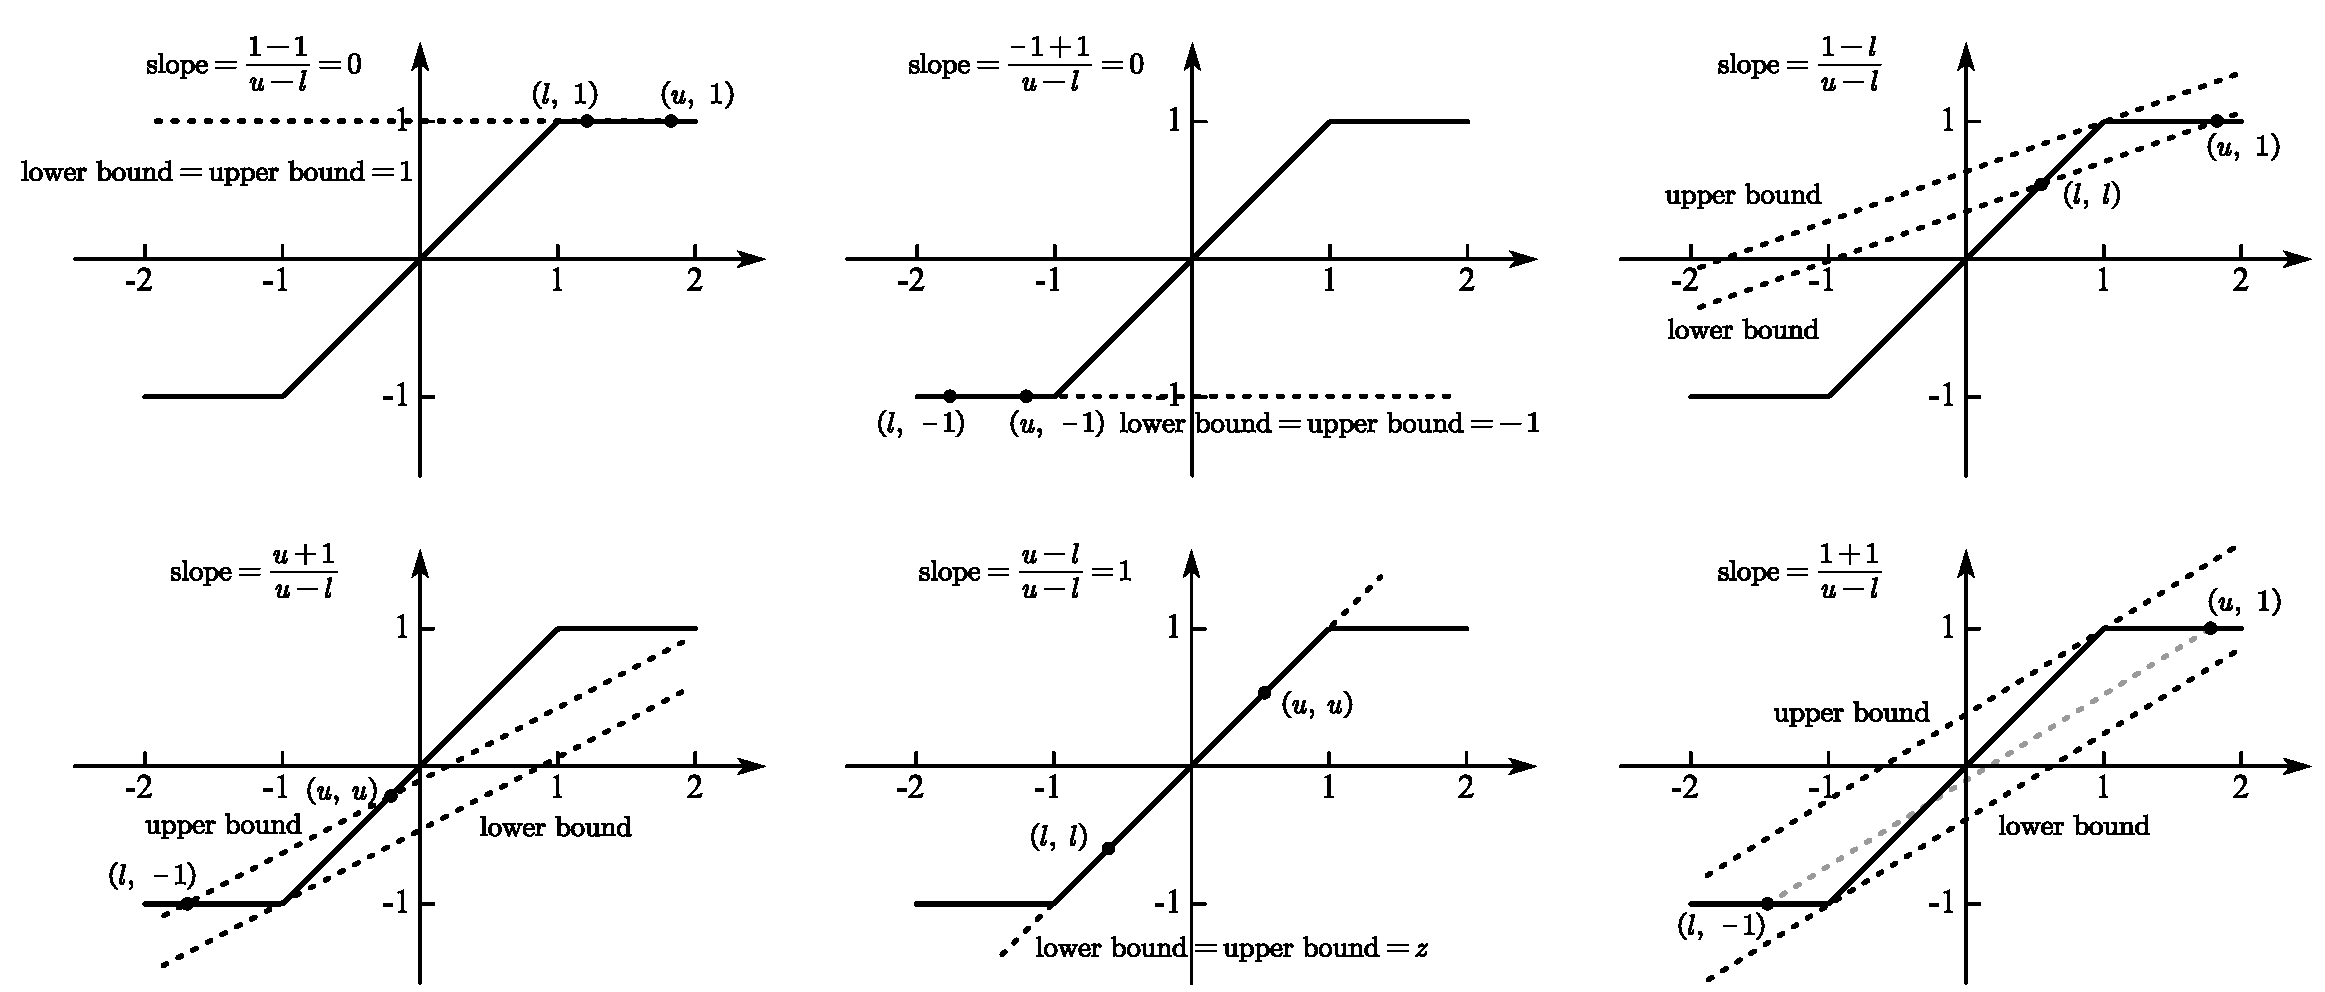
\includegraphics[width=\linewidth]{crown}
		\caption{}
		\label{fig:crown}
	\end{figure}
	
	Then, we can work out the interception of the lower bound is
	\begin{equation}
		\hardtanh{u} - \frac{\hardtanh{u} - \hardtanh{l}}{u - l} \hardtanh{u}
	\end{equation}
	and the interception of the upper bound is
	\begin{equation}
		\hardtanh{l} - \frac{\hardtanh{u} - \hardtanh{l}}{u - l} \hardtanh{l}
	\end{equation}

\item Implementation see \mintinline{python}|hardTanh_question.py|.

\item Noticed that
	\begin{equation}
		\hardtanh{z} = \relu{z + 1} - \relu{z - 1} - 1
	\end{equation}
	so it's not hard to find there are some cases can use the conclusion of the $\alpha$-CROWN discussion about $\relu{z}$, as illustrated in Figure \ref{fig:hardtanh_like_relu}.
	\begin{figure}[H]
		\centering
		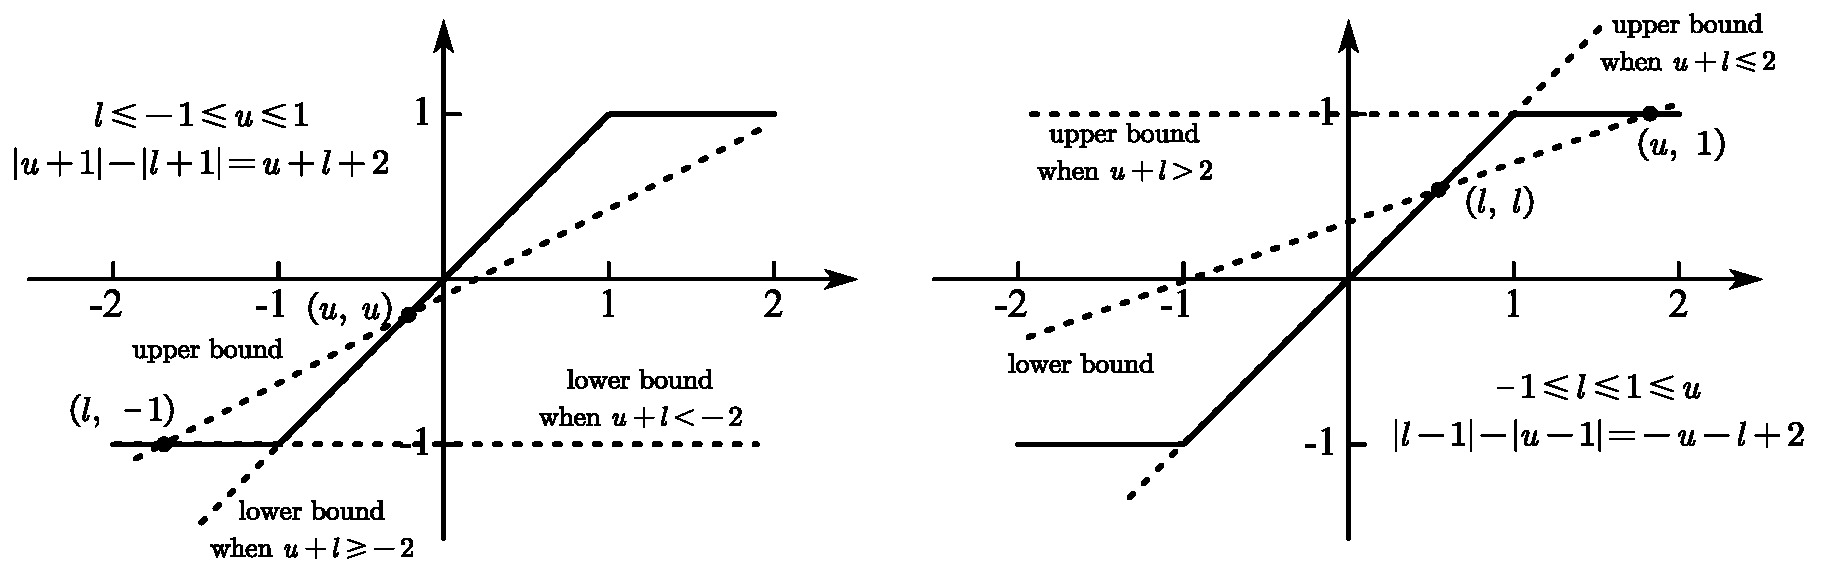
\includegraphics[width=\linewidth]{hardtanh_like_relu}
		\caption{Two Cases Similar to $\relu{z}$}
		\label{fig:hardtanh_like_relu}
	\end{figure}
	Now, we just need to focus on the most complicated case, which is $l < -1$ and $u > 1$.
	\begin{figure}[H]
		\centering
		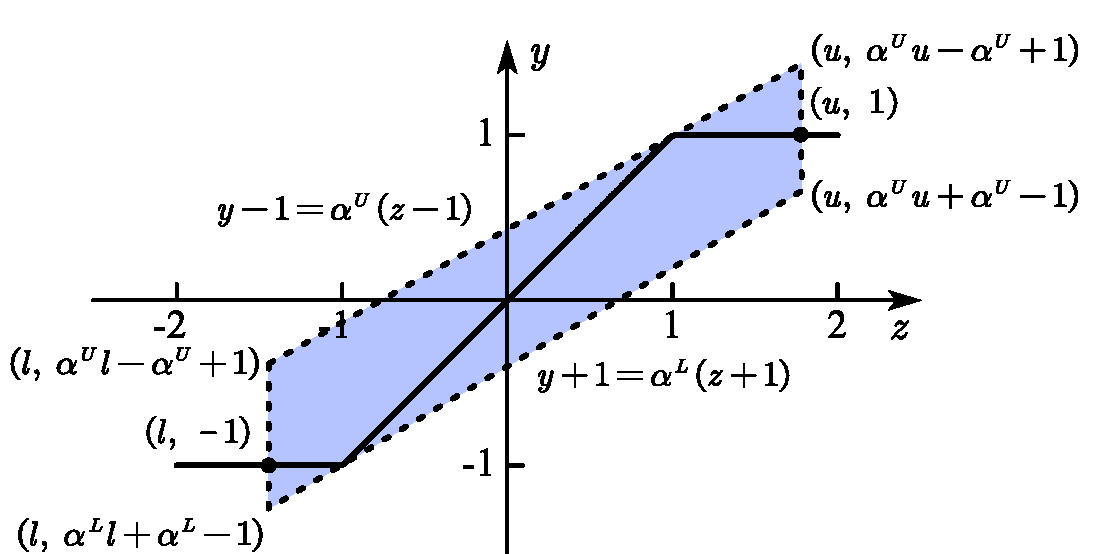
\includegraphics[width=0.6\linewidth]{hardtanh_comp_case}
		\caption{}
		\label{fig:hardtanh_comp_case}
	\end{figure} Suppose the linear bounds are
	\begin{equation}
		\alpha^{L} (z + 1) - 1 \leqslant \hardtanh{z} \leqslant \alpha^{U} (z - 1) + 1, \ l \leqslant z \leqslant u
	\end{equation}
	where 
	\begin{equation}
	\begin{gathered}
		0 \leqslant \alpha^{L} \leqslant \frac{\hardtanh{u} - \hardtanh{l}}{u - \hardtanh{l}} = \frac{2}{u + 1} < 1\\
		0 \leqslant \alpha^{U} \leqslant \frac{\hardtanh{u} - \hardtanh{l}}{\hardtanh{u} - l} = \frac{2}{1 - l} < 1
	\end{gathered}
	\end{equation}
	Then the area of the region enclosed by lines $z = l$, $z = u$, the lower and the upper bound is 
	\begin{equation}
		\operatorname{Area} = \frac{u - l}{2}\left[(u + l - 2) \alpha^{U} - (u + l + 2) \alpha^{L} + 4\right]
	\end{equation}
	Subsequently, 
	\begin{enumerate}[(a)]
		\item when $u + l - 2 \leqslant 0$ and $-u - l - 2 \leqslant 0$, i.e. $-2 \leqslant u + l \leqslant 2$, to minimize the area, we should let $\alpha^{L} = \dfrac{2}{u + 1}$ and $\alpha^{U} = \dfrac{2}{1 - l}$;
		
		\item when $u + l - 2 \leqslant 0$ and $-u - l - 2 > 0$, i.e. $u + l > 2$, to minimize the area, we should let $\alpha^{L} = \dfrac{2}{u + 1}$ and $\alpha^{U} = 0$;
		
		\item when $u + l - 2 > 0$ and $-u - l - 2 \leqslant 0$, i.e. $u + l < -2$, to minimize the area, we should let $\alpha^{L} = 0$ and $\alpha^{U} = \dfrac{2}{1 - l}$;
		
		\item it impossible for both $u + l - 2 > 0$ and $-u - l - 2 > 0$ to hold simultaneously.
	\end{enumerate}
	This implies
	\begin{equation}
		\alpha^{L} = \begin{cases}
			\dfrac{2}{u + 1}, \ u + l \geqslant -2\\
			0, \ u + l < -2
		\end{cases}, \alpha^{U} = \begin{cases}
			\dfrac{2}{1 - l}, \ u + l  \leqslant 2\\
			0, \ u + l > 2
		\end{cases}, \ l < -1, \ u > 1
	\end{equation}
	In fact, the conclusion above is consistent with cases in Figure \ref{fig:hardtanh_like_relu}. What's more, it's not hard to check the conclusion is even consistent with other cases. Specifically, we have
	\begin{equation}
	\begin{gathered}
		\alpha^{L} = \begin{cases}
			\dfrac{\hardtanh{u} - \hardtanh{l}}{u - \hardtanh{l}}, \ u + l \geqslant -2\\
			0, \ u + l < -2
		\end{cases}\\
		 \alpha^{U} = \begin{cases}
			\dfrac{\hardtanh{u} - \hardtanh{l}}{\hardtanh{u} - l}, \ u + l  \leqslant 2\\
			0, \ u + l > 2
		\end{cases}
	\end{gathered}
	\end{equation}
	Finally, we can work out the interception of the lower bound is
	\begin{equation}
	\begin{cases}
		\hardtanh{l} - \dfrac{\hardtanh{u} - \hardtanh{l}}{u - \hardtanh{l}} \hardtanh{l}, \ u + l \geqslant -2\\
		\hardtanh{l}, \ u + l < -2, \ \text{(actually is -1, since} \ 2 l < u + l < -2 \ \Rightarrow \ l < -1 \text{)}
	\end{cases}
	\end{equation}
	and the interception of the upper bound is
	\begin{equation}
	\begin{cases}
		\hardtanh{u} - \dfrac{\hardtanh{u} - \hardtanh{l}}{u - \hardtanh{l}} \hardtanh{u}, \ u + l \leqslant 2\\
		\hardtanh{u}, \ u + l > 2, \ \text{(actually is 1, since} \ 2 u > u + l > 2 \ \Rightarrow \ u > 1 \text{)}
	\end{cases}
	\end{equation}

\item Implementation see \mintinline{python}|hardTanh_question_alpha.py|. Results for CROWN and $\alpha$-CROWN is shown in Table \ref{tab:CROWN} and Table \ref{tab:alpha_CROWN} respectively. Experimental logs can also be checked in the folder.

\begin{minipage}[l]{0.48\linewidth}
	\begin{table}[H]
		\centering
		\caption{Lower and Upper CROWN Bounds}
		\begin{tabular}{ccc}
			\toprule
			& Lower Bound & Upper Bound \\
			\midrule
			$f_0$ & -5.8888 & 7.9799 \\
			$f_1$ & -8.4223 & 3.8257 \\
			$f_2$ & -7.1542 & 6.6943 \\
			$f_3$ & -4.233 & 10.6406 \\
			$f_4$ & -12.0069 & -0.582 \\
			$f_5$ & -13.1308 & 2.7378 \\
			$f_6$ & -15.1046 & -1.7304 \\
			$f_7$ & 6.1154 & 21.6736 \\
			$f_8$ & -6.8795 & 6.2323 \\
			$f_9$ & -5.9975 & 6.5901 \\
			\bottomrule
		\end{tabular}
		\label{tab:CROWN}
	\end{table}
\end{minipage}
\begin{minipage}[r]{0.48\linewidth}
	\begin{table}[H]
		\centering
		\caption{Lower and Upper $\alpha$-CROWN Bounds}
		\begin{tabular}{ccc}
			\toprule
			& Lower Bound & Upper Bound \\
			\midrule
			$f_0$ & -5.2428 & 7.3142 \\
			$f_1$ & -8.3839 & 2.5022 \\
			$f_2$ & -7.0532 & 4.9316 \\
			$f_3$ & -3.1677 & 9.9903 \\
			$f_4$ & -11.7056 & -1.1283 \\
			$f_5$ & -12.3369 & 2.3594 \\
			$f_6$ & -14.153 & -2.3708 \\
			$f_7$ & 6.1764 & 20.4607 \\
			$f_8$ & -6.1789 & 5.2903 \\
			$f_9$ & -5.2493 & 5.474 \\
			\bottomrule
		\end{tabular}
		\label{tab:alpha_CROWN}
	\end{table}	
\end{minipage}	

It's clear that the $\alpha$-CROWN bounds are tighter than CROWN Bounds.
\end{enumerate}

\end{document}
